\documentclass[9pt]{article}
 \usepackage{amsmath}
 \usepackage{amssymb}
 \usepackage{graphicx}    % needed for including graphics e.g. EPS, PS \usepackage{tikz}
 \usepackage{tikz}
 \usepackage{relsize}
 \usetikzlibrary{patterns,decorations.pathreplacing,shapes,arrows}
 \usepackage{algorithm2e}
 \topmargin -2.5cm        % read Lamport p.163
 \oddsidemargin -0.04cm   % read Lamport p.163
 \evensidemargin -0.04cm  % same as oddsidemargin but for left-hand pages
 \textwidth 16.59cm
 \textheight 25.94cm
% \pagestyle{empty}        % Uncomment if don't want page numbers
 \pagenumbering{gobble}
 \parskip 7.2pt           % sets spacing between paragraphs
 %\renewcommand{\baselinestretch}{1.5} 	% Uncomment for 1.5 spacing between lines
 \parindent 0pt		  % sets leading space for paragraphs

% No date in header
\date{}

\newcommand{\lp}{\left(}
\newcommand{\rp}{\right)}
\newcommand{\lb}{\left[}
\newcommand{\rb}{\right]}
\newcommand{\ls}{\left\{}
\newcommand{\rs}{\right\}}
\newcommand{\lbar}{\left|}
\newcommand{\rbar}{\right|}
\newcommand{\ld}{\left.}
\newcommand{\rd}{\right.}

\newcommand{\myexists}{\exists \hspace{.3mm}}

\newcommand{\hs}{\hspace{.75mm}}
\newcommand{\bs}{\hspace{-.75mm}}
\newcommand{\nin}{\noindent}

\newcommand{\fx}{f\bs\left( x \right)}
\newcommand{\gx}{g\bs\left( x \right)}
\newcommand{\qx}{q\bs\left( x \right)}

\newcommand{\nn}{\nonumber}

\newcommand{\vfive}{\vspace{5mm}}
\newcommand{\vthree}{\vspace{3mm}}

\newcommand{\fof}[1]{f\lp #1\rp}
\newcommand{\gof}[1]{g\lp #1\rp}
\newcommand{\qof}[1]{q\lp #1\rp}

\newcommand{\myp}[1]{\left( #1 \right)}
\newcommand{\myb}[1]{\left[ #1 \right]}
\newcommand{\mys}[1]{\left\{ #1 \right\}}
\newcommand{\myab}[1]{\left| #1 \right|}

\newcommand{\myj}{_j}
\newcommand{\myjp}{_{j+1}}
\newcommand{\myjm}{_{j-1}}

\newcommand{\f}[1]{f\hspace{-1mm}\left( #1 \right)}
\newcommand{\fp}[1]{f'\hspace{-1mm}\left( #1 \right)}
\newcommand{\g}[1]{g\hspace{-1mm}\left( #1 \right)}
\newcommand{\gp}[1]{g'\hspace{-1mm}\left( #1 \right)}
\newcommand{\q}[1]{q\hspace{-1mm}\left( #1 \right)}
\newcommand{\qp}[1]{q'\hspace{-1mm}\left( #1 \right)}
\newcommand{\Px}[1]{P\hspace{-1mm}\left( x_{#1} \right)}
\newcommand{\Qx}[1]{Q\hspace{-1mm}\left( x_{#1} \right)}

\newcommand{\tten}[1]{\times 10^{#1}}

\newcommand{\aij}[1]{a_{#1}}
\newcommand{\bij}[1]{b_{#1}}
\newcommand{\rij}[1]{r_{#1}}

\newcommand{\R}[1]{\mathbb{R}^{#1}}

\newcommand{\ith}{i^{\textrm{th}}}
\newcommand{\jth}{i^{\textrm{th}}}
\newcommand{\kth}{i^{\textrm{th}}}

\newcommand{\inv}[1]{{#1}^{-1}}

\newcommand{\bx}{\mathbf{x}}
\newcommand{\bv}{\mathbf{v}}
\newcommand{\bw}{\mathbf{w}}
\newcommand{\by}{\mathbf{y}}
\newcommand{\bb}{\mathbf{b}}
\newcommand{\be}{\mathbf{e}}
\newcommand{\br}{\mathbf{r}}
\newcommand{\xhat}{\hat{\mathbf{x}}}

\newcommand{\beq}{\begin{eqnarray}}
\newcommand{\eeq}{\end{eqnarray}}

\newcommand{\ben}{\begin{enumerate}}
\newcommand{\een}{\end{enumerate}}

\newcommand{\bsq}{\mathsmaller{\blacksquare}}

\newcommand{\iter}[1]{^{\myp{#1}}}

% matrix macro
\newcommand{\mymat}[1]{
\left[
\begin{array}{rrrrrrrrrrrrrrrrrrrrrrrrrrrrrrrrrrrrrrr}
#1
\end{array}
\right]
}

\newcommand{\smallaug}[1]{
\left[
\begin{array}{rr|r}
#1
\end{array}
\right]
}


% Actual document starts here
% ======================================================================================
\begin{document}

\begin{minipage}{0.65\textwidth}
\nin {\bf Numerical Analysis -- Fall 2023 } \\

{\bf \underline{Name:} Zane Perry}  %Replace 'XXXXXXX  XXXXXXX' in the previous { } with your name\\
{\bf \underline{Student ID:} 110075979}  %Replace 'ZZZZZZZZZ' in the previous { } with your Student ID
\end{minipage}\hfill
\begin{minipage}{0.35\textwidth}
\hfill {\bf Homework 1}%Replace the 'N' with the appropriate homework number} \\

\end{minipage}

% Actual text body starts here
% ======================================================================================

\vfive
===================================================================
\newline
\newline
\newline

% ===============================================
\ben
\item Problem 1
   
   Consider the polynomial: 
   
   $$p(x) = (x-2)^9 = x^9 -18x^8 + 144x^7 - 672x^6 + 2016x^5 - 4032x^4 + 5376x^3 - 4608x^2 + 2304x - 512$$
   
   
   i. If you were to plot $p(x)$ for the range $x = [1.920: 0.001: 2.080]$ using the fully expanded form above:
   
   \begin{center}
   	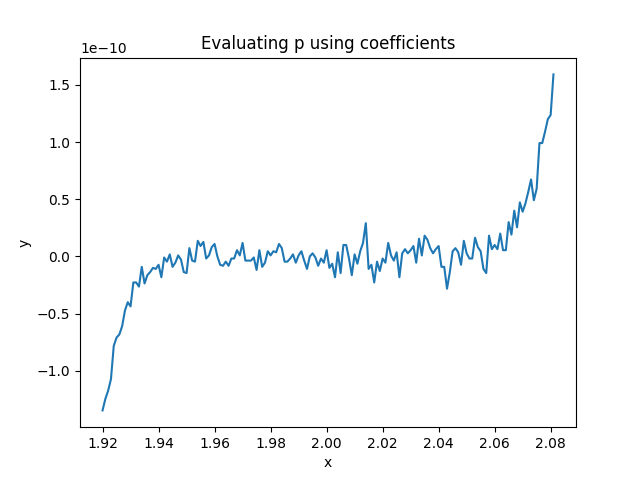
\includegraphics[scale=0.5]{1i}
   \end{center}
   
   
   ii. If you were instead to plot $p(x)$ for the same range using the factored binomial form above:
   
   \begin{center}
   	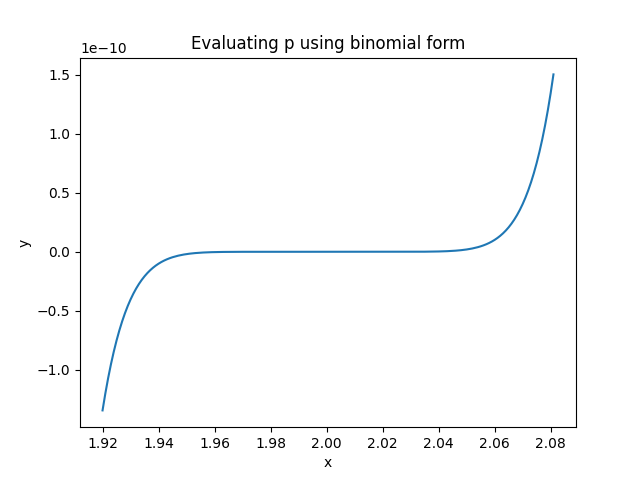
\includegraphics[scale=0.5]{1ii}
   \end{center}
   
   iii. The difference between these two plots is that the plot created using the expanded coefficient form of $p(x)$ is much more jagged than the plot created using the factored binomial form, which appears smooth along the entire curve. The discrepancy is caused by the fact that the fully expanded form contains many addition and subtraction operations with very long decimals. These long decimals result from the high power of the exponents on each individual term of the expression, where each successive multiplication results in further decimal points being calculated (due to the fact that decimal values are the input). When these decimal points are then added or subtracted to each other, there are multiple opportunities for the decimals to be truncated, resulting in a less accurate final answer. The binomial form on the other hand only has a single subtraction operation followed by the exponent, resulting in much less opportunities for decimal truncation. Therefore, because there are less computer operations overall in the binomial form of $p(x)$, and less chances for decimal truncation, the correct plot of this function is the second one, for $p(x) = (x-2)^9$.
   

\newpage

\item Problem 2


	i. Evaluate $\sqrt{x+1} - 1$ for $x \simeq 0$
	$\\$
	$\\$
	In the expression above, when $x$ is close to zero, the expression under the square root sign would evaluate to a number close to 1. When 1 is then subtracted from this, there is a risk of the two expressions cancelling to zero despite not being equal. Therefore, the subtraction is the part of the expression that needs to be avoided:
	
	\begin{align*}
		\sqrt{x+1} - 1 &=  \sqrt{x+1} - 1 \cdot \frac{\sqrt{x+1} + 1}{\sqrt{x+1} + 1}  \; \; \; \; \text{(using conjugate)} \\
		&= \frac{(x + 1) - 1}{\sqrt{x+1} + 1} \\
		&= \frac{x}{\sqrt{x+1} + 1}
	\end{align*}
	
	
	The new expression does not have any subtraction at all, and therefore the problem described above of possible cancellation due to subtraction would not be present.
	
	$\\$
	
	ii. Evaluate $\sin{(x)}-\sin{(y)}$ for $x \simeq y$
	
	$\\$
	
	iii. Evaluate $\frac{1 - \cos{(x)}}{\sin{(x)}}$ for $x \simeq 0$
	
	$\\$
	In the expression above, the risk of cancellation lies in the $1-\cos{(x)}$ term as the cosine would evaluate to a number close to 1 when $x$ is close to 0. Therefore that subtraction is the term that needs to be avoided:
	
	\begin{align*}
		\frac{1 - \cos{(x)}}{\sin{(x)}} &= \frac{1 - \cos{(x)}}{\sin{(x)}} \cdot \frac{1 + \cos{(x)}}{1 + \cos{(x)}} \; \; \; \text{(using conjugate)}\\
		&= \frac{1 - \cos^2{(x)}}{\sin{(x)}(1 + \cos{(x)})} \\
		&= \frac{\sin^2{(x)}}{\sin{(x)}(1 + \cos{(x)})} \; \; \; \text{(using trig identities)}\\
		&= \frac{\sin{(x)}}{1 + \cos{(x)}}
	\end{align*}
	
	The new expression does not have any subtraction at all, and therefore the problem described above of possible cancellation due to subtraction would not be present.
	
	
	
	
\newpage


\item Problem 3

$\\$

Let $f(x)=(1+x+x^3)\cos{(x)}$

$\\$

In order to find the 2nd degree Taylor polynomial about $x_0 = 0$, we can use the formula for a Taylor polynomial:


$$P_2(x) = f(x_0) + f'(x_0)x + \frac{f''(x_0)}{2!}x^2$$

Which will have an error lying in the third term of the polynomial:

$$R_2(x) = \frac{M}{3!}x^3$$

Where $M$ is a maximum upper bound of $f'''(x)$ in the range of $[x_0, x]$

Solving for the relevant coefficients and plugging into the Taylor formula:

\begin{align*}
	f(x) &= (1 + x + x^3)\cos{(x)} \\
	f'(x) &= (1 + 3x^2)\cos{(x)} - (1 + x + x^3)\sin{(x)}\\
	f''(x) &= 6x\cos{(x)} - (1 + 3x^2)\sin{(x)} - (1 + x + x^3)\cos{(x)} - (1 + 3x^2)\sin{(x)} \\
	&= 6x\cos{(x)} - (2+6x^2)\sin{(x)} - (1 + x + x^3)\cos{(x)} \\
	f'''(x) &= 6\cos{(x)} - 6x\sin{(x)} - 12x\sin{(x)} - (2 + 6x^2)\cos{(x)} + (1 + x + x^3)\sin{(x)} - (1 + 3x^2)\cos{(x)} \\ 
	&= 3\cos{(x)} + \sin{(x)} - 17x\sin{(x)} - 9x^2\cos{(x)} + x^3\sin{(x)}
\end{align*}


\begin{align*}
	f(x_0=0) &= 1 \\
	f'(x_0=0) &= 1 - 0 = 1 \\
	f''(x_0=0) &= 0 - 0 - 1 = -1
\end{align*}

$$P_2(x) = 1 + x - \frac{1}{2}x^2$$


	\ben
	
	\item We can use $P_2(x)$ to approximate $f(0.5)$
	\begin{align*}
		P_2(0.5) &= 1 + \frac{1}{2} - \frac{1}{2}\left( \frac{1}{2} \right)^2 \\
		&= \frac{11}{8}
	\end{align*}
	
	We can use the error formula listed above in order to estimate an upper bound on the error of this approximation:
	
	\item
	
	\item We can also use $P_2(x)$ to estimate $\int_0^1 f(x) dx$
	
	\begin{align*}
		\int_0^1 P_2(x)dx &= \int_0^1 1 + x - \frac{1}{2}x^2 dx \\
		&= \left[ x + \frac{1}{2}x^2 - \frac{1}{6}x^3 \right]_0^1 \\
		&= \left( 1 + \frac{1}{2} - \frac{1}{6} \right) - (0) \\
		&= \frac{4}{3}
	\end{align*}
	
	\item
	
	\een



\newpage

\item Problem 4


$\\$

	Consider the quadratic equation $ax^2+bx+c=0$ with $a=1$, $b=-56$, and $c=1$
	
	\ben
	
	\item The roots of this quadratic can be found using the standard formula:
	
	$$r_{1,2} = \frac{-b \pm \sqrt{b^2 - 4ac}}{2a}$$
	
	If the square root can only be computed correctly to 3 decimals, the following roots are computed for the given quadratic:
	
	\item
	
	\een



\newpage

\item Problem 5

$\\$

Consider computing $y=x_1 - x_2$ with $\tilde{x_1} = x_1 + \Delta x_1$ and $\tilde{x_2} = x_2 + \Delta x_2$. If the operation $x_1 - x_2$ is carried out exactly we get $\tilde{y} = y + \Delta y$ where $\Delta y = \Delta x_1 - \Delta x_2$



	\ben 
	
	\item
	
	\item
	
	\item
	
	
	\een


\een

\end{document}
